\important{Focus sur: la centrale hydraulique}

\begin{center}
    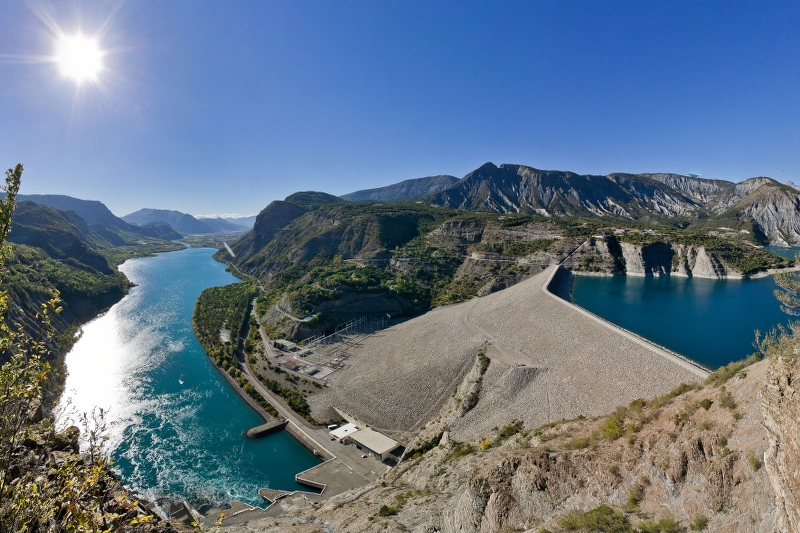
\includegraphics[width=6cm]{images/barrage.jpg}

    \textit{Barrage hydroélectrique de Serre-Ponçon (Hautes-Alpes)}
\end{center}


Une centrale hydraulique est un dispositif qui permet de produire de l'électricité à partir de la force de l'eau. Elle est le plus souvent installée au pied d'un barrage qui retient une grande quantité d'eau en hauteur, par exemple dans une vallée de montagne.
Quand on ouvre les vannes du barrage, l'eau s'écoule rapidement vers le bas et fait tourner une turbine. Cette turbine entraîne un alternateur qui produit de l'électricité.
L'avantage est qu'on peut décider à tout moment d'ouvrir ou de fermer les vannes : la production d'électricité s'adapte facilement aux besoins.

La centrale hydraulique utilise l'eau, une source d'énergie renouvelable, et ne rejette pas de CO\textsubscript{2}. Sa production est forte et peut être adaptée à la demande.
La construction d'un barrage nécessite un relief adapté (montagnes ou grandes rivières), et noie une partie de la vallée, ce qui transforme le paysage et perturbe la vie des animaux et des poissons.